\documentclass{article}

\usepackage{coursenotes}

\set{AuthorName}{TC Fraser}
\set{Email}{tcfraser@tcfraser.com}
\set{Website}{www.tcfraser.com}
\set{ClassName}{Stochastic Processes}
\set{School}{University of Waterloo}
\set{CourseCode}{Stat 433}
\set{InstructorName}{Yi Shen}
\set{Term}{Fall 2016}
\set{Version}{1.0}

\draftprofile[TC Fraser]{TC}{Purple}
\newcommand{\val}[1]{X_{#1} = x_{#1}}

\begin{document}

\titlePage

\tableOfContents

\disclaimer

\section{DTMC}

\subsection{Review of Probability}

A \term{random variable (r.v.)}  $X$ is a real valued function of the outcomes of a random experiment.

\[ X : \Om \to R \]

Where $\Om = \bc{\w_1, \w_2, \ldots}$ is the \term{sample space} corresponding to all possible outcomes $\w_i$. The outcomes can in principle be any objects (numbers, strings, etc.). We say that $X$ maps each outcome $\w$ to a real number $\w \mapsto X\br{\w} \in \R$. \\

A \term{stochastic process} is a family of random variables $\bc{X_t}_{t \in T}$, defined on a common sample space $\Om$. $T$ is referred to as the index set for the stochastic process which is often understood as time. The index set $T$ can take a discrete spectrum,
\[ T = \bc{0, 1, 2, \ldots} \qquad \bc{X_n \mid n = 0, 1, 2, \ldots} \]
Alternatively, $T$ can take on a continuous spectrum,
\[ T = \bc{t \mid t \geq 0} = \left[ 0 , \inf \right) \]

The \term{state space} $S$ is the collection of all possible values of $X_t$'s. It is important to understand the distinction of between sample space and state space. Additionally, the state space can either have discrete or continuous spectrum. \\

A question remains, \textit{Why do we need the family of random variables to be defined on a common sample space?} The answer being that we would like to be able to discuss the joint behaviour of $X_t$'s. If $X_1$ has domain $\Om_1$ and $X_2$ has domain $\Om_2$ (where $\Om_1 \neq \Om_2$), then one can \textit{not} talk about common ideas of correlations and associations between $X_1$ and $X_2$. As such we assert that all members of a stochastic process share the same sample space domain $\Om$.

\subsection{Discrete-time Markov Chain}

A \term{discrete-time stochastic process} $\bc{X_n \mid n \in 0, 1, 2, \ldots}$ is said to be a \term{Discrete-time Markov Chain (DTMC)}  if the following conditions hold:
\begin{enumerate}
    \item The state space is at most \textit{countable}\footnote{Countable meaning there is a one-to-one mapping from the state space to the natural numbers.} (i.e. finite or countable).
    \[ S = \bc{0, 1, \ldots, k} \quad \textrm{or} \quad S = \bc{0, 1, 2, \ldots} \]
    \item \term{Markov Property}: For any $n = 0, 1, 2, \ldots$,
    \[ P\br{X_{n+1} = x_{n+1} \mid X_n = x_n, X_{n-1} = x_{n-1}, \ldots, X_{0} = x_{0}} = P\br{X_{n+1} = x_{n+1} \mid X_{n} = x_{n}} \]
\end{enumerate}
We use capital letters $X$ to denote the random variable and lower case letters $x$ to denote a specific realization or valuation of $X$. The motivation of the Markov property is that future events $X_{n+1} = x_{n+1}$ are independent of past histories $\bc{X_{i} = x_{i} \mid i = 0, 1, \ldots, n-1}$ given the immediate past state $X_{n} = x_{n}$. The intuition being that the future and the past are probabilistically independent.

\begin{center}
    \textit{Given the present, the future and the past are independent.}
\end{center}

\subsection{Transition Probability}

The \term{transition probability} from a state $i \in S$ at time $n$ to state $j \in S$ (at time $n+1$) is given by,
\[ P_{n, i, j} \defined P \br{X_{n+1}= j \mid X_{n} = i} \qquad n = 0, 1, 2, \ldots \eq \label{eq:trans_prob}\]
In full generality, the transition probability could depend on time $n$ but in this course we will restrict ourselves to transition probabilities that \textit{do not} depend on time $n$ ($P_{n, i, j} = P_{i, j}$). We say that the MC is \term{(time-)homogeneous} if this property holds. From now on, this will be our default setting. \\

The matrix of all transition probabilities $P = \bc{P_{i,j} \mid i,j \in S}$ is called the \term{one-step transition (probability) matrix} for $\bc{X_{n} \mid n \in T}$.
\[ P = \begin{pmatrix}
P_{00} & P_{01} & \cdots & P_{0j} & \cdots \\
P_{10} & P_{11} & \cdots & P_{1j} & \cdots \\
\vdots & \vdots & \ddots & \vdots & \cdots \\
P_{i0} & P_{i1} & \cdots & P_{ij} & \cdots \\
\vdots & \vdots & \vdots & \vdots & \ddots
\end{pmatrix} \]
The one-step transition matrix $P$ has the following properties,
\[ P_{i,j} \geq 0 \eq \label{eq:trans_positive_entries} \]
\[ \forall i : \sum_{j \in S} P_{ij} = 1 \eq \label{eq:trans_row_sum}\]
The entries are non-negative because they represent probabilities and the row sums for $P$ are always unitary.\\

The \term{n-step transition probability} is defined via the homogeneous property,
\[ \forall i,j \in S : P_{ij}^{(n)} \defined P\br{X_{n+m} = j \mid X_{n} = i} = P\br{X_{n} = j \mid X_{0} = i} \]
Analogously, the \term{n-step transition matrix} is the matrix,
\[ P^{(n)} = \bc{P_{ij}^{(n)} \mid i, j \in S} \]

\begin{theorem}
There is a simple relation between the n-step transition matrix $P^{(n)}$ and the one step transition matrix $P$.
\[ P^{(n)} = P^{(n-1)} \cdot P = \underbrace{P \cdot P \cdot \cdots \cdot P}_{n} = P^n \]
\end{theorem}

\begin{proof}
Proof by induction:
\[ P^{(1)} = P \note{By definition.} \]
We also have $P^{(0)} = P^{0} = \mathbb{I}$ is the identity matrix. We now assume $P^{(n)} = P^{n}$. Then $\forall i,j \in S$,
\begin{align*}
    P_{ij}^{(n+1)} &= P\br{X_{n+1} = j \mid X_{0} = i} \\
    &= \sum_{k \in S} P\br{X_{n+1} = j, X_{n} = k \mid X_{0} = i} \note{Total probability}\\
    &= \sum_{k \in S} \f{P\br{X_{n+1} = j, X_{n} = k, X_{0} = i}}{P\br{X_{0} = i}} \\
    &= \sum_{k \in S} \f{P\br{X_{n+1} = j, X_{n} = k, X_{0} = i}}{P\br{X_{n} = k, X_{0} = i}}\f{P\br{X_{n} = k, X_{0} = i}}{P\br{X_{0} = i}} \\
    &= \sum_{k \in S} P\br{X_{n+1} = j \mid X_{n} = k, X_{0} = i} \cdot P\br{X_{n} = k \mid X_{0} = i} \note{Conditional total probability}\\
    &= \sum_{k \in S} P\br{X_{n+1} = j \mid X_{n} = k} \cdot P\br{X_{n} = k \mid X_{0} = i} \note{Use Markov Property}\\
    &= \sum_{k \in S} P_{kj} \cdot P_{ik}^{(n)} \note{Matrix terms}\\
    &= \br{P \cdot P^{(n)}}_{ij} \note{Matrix product}\\
    &= \br{P^{n+1}}_{ij} \note{Inductive Hypothesis}
\end{align*}
There we have proved that $P^{(n+1)} = P^{n+1}$ and so we have a complete proof that $P^{(n)} = P^{n}$.\\
\end{proof}

\begin{corollary}
As a corollary, we have obtained that,
\[ P^{(n)} = P^{(m)} \cdot P^{(n-m)} \quad \forall 0 \leq m \leq n \]
Or equivalently the \textbf{Chapman-Kolmogorov Equation} or simply C-K equation,
\[ P^{(n)}_{ij} = \sum_{k \in S} P^{(m)}_{ik} P^{(n-m)}_{kj} \quad \forall i,j \in S, \forall 0 \leq m \leq n \eq \label{eq:ck_equation} \]
\end{corollary}

So far, we have only been discussing transition probabilities. We will now divert our attention to actual distributions for a stochastic process. \\

Let $\al_n = \br{\al_{n, 0}, \al_{n, 1}, \ldots}$ be the \term{probability distribution vector} for $X_n$ at time $n$.
\[ \al_{n,k} = P\br{X_n = k} \qquad \forall k \in S \]
Note that $\al_{n,k} \geq 0$ and $\sum_{k\in S} \al_{n, k} = 1$ and $n = 0, 1, 2,\ldots$. We also define the initial distribution $\al_0$,
\[ \al_0 = \br{P\br{X_0 = 0}, P\br{X_0 = 1}, \ldots} \]
\begin{theorem}
The transition probability matrix reveals the following relationship between the distribution $\al_n$ at time $n$ and the distribution $\al_0$ at time $0$,
\[ \al_n = \al_0 \cdot P^{n} \eq \label{eq:transition_dist}\]
\end{theorem}
\begin{proof}
The proof \cref{eq:transition_dist} is quite trivial:
\begin{align*}
    \forall j \in S \quad \al_{n, j} &= P\br{X_n = j} \\
     &= \sum_{i \in S} P\br{X_n = j \mid X_0 = i} \cdot P\br{X_0 = i} \\
     &= \sum_{i \in S} \al_{0, i} \cdot P_{ij}^{n} \\
     &= \al_{0, 0} \cdot P_{0j}^{n} + \al_{0, 1} \cdot P_{1j}^{n} + \ldots \\
     &= \br{\al_{0} \cdot P^{n}}_j
\end{align*}
\end{proof}
More generally, for any $n = 1, 2, \ldots$ the finite dimensional distribution can be obtained from the following process iterative process,
\begin{align*}
&\hspace{-0.5in}P\br{X_n=x_n, X_{n-1}=x_{n-1}, \ldots, X_{0}=x_{0}} = \\
&P\br{X_{0} = x_{0}} \cdot\\
&P\br{X_{1} = x_{1} \mid X_0 = x_0} \cdot\\
&P\br{\val{2} \mid \val{1}, \val{0}} \cdots \\
&P\br{\val{n} \mid \val{n-1}, \ldots, \val{0}}
\end{align*}
But by the Markov condition, it must be that,
\begin{align*}
&\hspace{-0.5in}P\br{X_n=x_n, X_{n-1}=x_{n-1}, \ldots, X_{0}=x_{0}} = \\
&P\br{X_{0} = x_{0}} \cdot\\
&P\br{X_{1} = x_{1} \mid X_0 = x_0} \cdot \\
&P\br{\val{2} \mid \val{1}} \cdots \\
&P\br{\val{n} \mid \val{n-1}}
\end{align*}
First recognize the first term on the RHS ($P\br{X_{0} = x_{0}} = \al_{0, x_0}$), and also the remaining terms are transition probabilities as per \cref{eq:trans_prob}. Therefore it must be that,
\[ P\br{X_n=x_n, X_{n-1}=x_{n-1}, \ldots, X_{0}=x_{0}} = \al_{0, x_0} P_{x_0x_1}P_{x_1x_2}\cdots P_{x_{n-1}x_n} \]
Even more generally, for $0 \leq t_1 < t_2 < \cdots < t_n$,
\[ P\br{\val{t_n}, \val{t_{n-1}}, \ldots, \val{t_{1}}} = P\br{\val{t_1}} \br{P^{t_2 - t_1}}_{x_{t_1}x_{t_2}}\br{P^{t_3 - t_2}}_{x_{t_2}x_{t_3}}\cdots\br{P^{t_{n} - t_{n-1}}}_{x_{t_{n-1}}x_{t_{n}}}  \]
Since $P\br{\val{t_1}} = \al_{t_1 x_{t_1}} = \sum_{k \in S} \al_{0, k} P^{t_1}_{k, x_{t_1}}$,
\[ \al_{t_1} = \al_{0} \cdot P^{t_1} \]
This means the probabilistic properties of a DTMC are fully characterized by two things:
\begin{enumerate}
    \item The initial distribution $\al_{0}$
    \item Transition matrix $P$
\end{enumerate}
\subsection{Classification of States}
\newcommand{\comm}{\leftrightarrow}
\newcommand{\acc}[2]{#1 \to #2}

State $j$ is \term{accessible} from state $i$ (denoted $\acc{i}{j}$) if there exists $n = 0, 1, \ldots$ such that $P^{(n)}_{ij} > 0$. Intuitively, one can transition from state $i$ to state $j$ in finite steps $n$ with positive probability. If $i$ is also accessible from $j$, then we say $i$ and $j$ \term{communicate}, denoted as ${i}\comm{j}$.
\[ {i}\comm{j} \Leftrightarrow \exists m, n \geq 0, P_{ij}^{(m)} > 0, P_{ji}^{(n)} > 0 \]
\begin{theorem}
The binary communication relation ``${}{\comm}$'' is in fact a equivalence relation:
\begin{itemize}
    \item Reflexivity ${i}\comm{i}$
    \item Symmetry ${i}\comm{j} \implies {j}\comm{i}$
    \item Transitivity ${i}\comm{j}, {j}\comm{k} \implies {i}\comm{k}$
\end{itemize}
\end{theorem}
\begin{proof}
First, reflexivity is easy to prove by definition. Let $n = 0$ and recognize that $P^{(0)}_{ii}$ has a certain probability by definition,
\[ P^{(0)}_{ii} = 1 \implies {i}\comm{i} \]
Second, symmetry follows by definition,
\[ P_{ij}^{(m)} > 0, P_{ji}^{(n)} > 0 \Leftrightarrow P_{ji}^{(n)} > 0, P_{ij}^{(m)} > 0 \]
Third, transitivity can be proving by letting $m$ and $n$ be the unknown quantifiers:
\[ \exists m \quad P_{ij}^{(m)} > 0, \exists n \quad P_{jk}^{(n)} > 0 \]
Then by the CK equation \cref{eq:ck_equation},
\[ P^{(m+n)}_{ik} = \sum_{l \in S} P^{(m)}_{il}P^{(n)}_{lk} \]
Let $l = j$ be a single, fixed entry in the summation,
\[ P^{(m+n)}_{ik} \geq P^{(m)}_{ij}P^{(n)}_{jk} > 0 \]
Therefore we have that $k$ is accessible from $i$ ($\acc{i}{j}$). Analogously we have that $\acc{i}{j}$ therefore ${i}\comm{k}$. \\
\end{proof}
The communication equivalence relations then divides the state space $S$ into different equivalence classes. That is, the states in one class comm with each other; the states in different classes do not comm. The equivalent classes form a \textit{partition} of the state space $S$. \\

The family $\bc{S_1, S_2, \ldots S_n}$ is a \term{partition} of $S$ if,
\begin{enumerate}
    \item $S_i \subset S \mid \forall i \in 1,2,\ldots,n$
    \item $S_i \cap S_j \neq \emptyset$ for all $i \neq j$
    \item $\bigcup_{i} S_i = S$
\end{enumerate}

We can find the equivalent classes by drawing a graph where the states in $S$ are the nodes of the graph and a directed edge is placed going from $i$ to $j$ if $j$ is accessible from $i$ in one-step: $P_{ij} > 0$. Then identifying the the equivalent classes corresponds to identifying the loops of this graph within one step. \\

\begin{example}

As an example, consider the transition matrix $P$ as follows.

\[ P = \kbordermatrix{
    & 0 & 1 & 2 & 3 & 4 \\
    0& 0.2 & 0.8 & 0 & 0 & 0 \\
    1& 0.6 & 0.4 & 0 & 0 & 0 \\
    2& 0 & 0.5 & 0 & 0.5 & 0 \\
    3& 0 & 0 & 0 & 0.7 & 0.3 \\
    4& 0 & 0 & 0 & 0.1 & 0.9} \]

The associated one-step accessibility graph is then,
\begin{center}
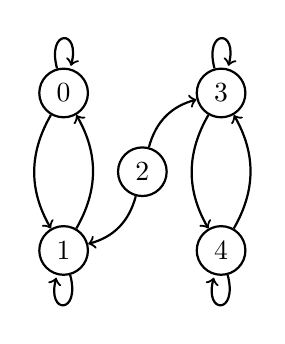
\begin{tikzpicture}
    \begin{scope}
        \tikzstyle{every node}=[fill=white, draw=black, circle, thick, text=black, scale=1.0]
        \node (0) at (0,2) {$0$};
        \node (1) at (0,0) {$1$};
        \node (2) at (1,1) {$2$};
        \node (3) at (2,2) {$3$};
        \node (4) at (2,0) {$4$};
    \end{scope}
    \begin{scope}
        \tikzstyle{every edge}=[draw, thick, ->]
        \path
        (0) edge[bend right] (1)
        (1) edge[bend right] (0)
        (0) edge[loop above] (0)
        (1) edge[loop below] (1)
        (3) edge[bend right] (4)
        (4) edge[bend right] (3)
        (3) edge[loop above] (3)
        (4) edge[loop below] (4)
        (2) edge[bend left] (3)
        (2) edge[bend left] (1);
    \end{scope}
\end{tikzpicture}
\end{center}

Where the loops of $S = \bc{0,1,2,3,4}$ form the following partition,
\[ S_1 = \bc{0,1} \quad S_2 = \bc{2} \quad S_3 = \bc{3, 4} \]
\end{example}

These equivalent classes are useful for Markov chains because it allows one to separate the behaviour of the equivalence classes and study them individually. A MC which has only one equivalent class is called \term{irreducible}. \\

Furthermore, let us define the \term{period} of state $i$ as,

\[ d\br{i} = \gcd \bc{n \in \Z^{+} \mid P_{ij}^{n} > 0} \]

Additionally, if $P_{ii}^{n} = 0$ holds for all $n > 0$, we say that $d\br{i} = \inf$. If the period of $i$ happens to be $d\br{i} = 1$ then the state $i$ is said to be \term{aperiodic}. Alternatively, locus of steps that we can go back by are \textit{co-prime}. A MC is called aperiodic if all its states $S$ are aperiodic.\\

The period of a state is useful do to the following theorem,

\begin{theorem}
\label{thm:period_class_prop}
The period of a state is a class property. If ${i}\comm{j}$, then $d\br{i} = d\br{j}$.
\end{theorem}

\begin{proof}
If $i = j$ we are already done. If $i \neq j$, since ${i}\comm{j}$, then $\exists n, m$ such that,
\[ P_{ij}^{n} > 0 \quad P_{ji}^{m} > 0 \]
Then for any $l$ such that $P^{l}_{jj} > 0$,
\[ P_{ii}^{n+m+l} \geq P_{ij}^{n}P_{jj}^{l}P_{ji}^{m} \eq \label{eq:period_class_prop_2} \]
Because $P_{ij}^{n}P_{jj}^{l}P_{ji}^{m}$ happens to be a specific way for $P_{ii}^{n+m+l}$ to occur. Since ${i}\comm{j}$ and $l$ was chosen carefully,
\[ P_{ii}^{n+m+l} > 0 \]
Moreover, we also have that,
\[ P_{ii}^{n+m} \geq P_{ij}^{n}P_{ji}^{m} \eq \label{eq:period_class_prop_1}\]
Since $d\br{i}$ divides both $n+m$ and $n+m+l$ by \cref{eq:period_class_prop_1,eq:period_class_prop_2}, then $d\br{i}$ also divides $l$. This holds for all $l$ such that $P_{ii}^{l}>0$. This implies that $d\br{i}$ is a common divisor of $\bc{l \mid P_{jj}^{l} > 0}$ an thus $d\br{i}$ divides,
\[ d\br{j} = \gcd \bc{l \mid P_{jj}^{l} > 0} \]
By symmetry $d\br{j}$ divides $d\br{i}$. Therefore $d\br{i} = d\br{j}$. \\
\end{proof}

\begin{remark}
It is important to note that $d\br{i} = k \not\Rightarrow P_{ii}^{(k)} > 0$. As a counterexample consider the following one step accessibility graph,
\begin{center}
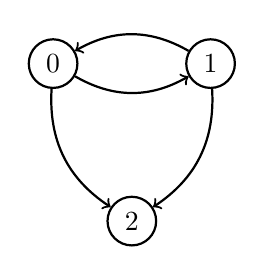
\begin{tikzpicture}
    \begin{scope}
        \tikzstyle{every node}=[fill=white, draw=black, circle, thick, text=black, scale=1.0]
        \node (0) at (-1,2) {$0$};
        \node (1) at (1,2) {$1$};
        \node (2) at (0,0) {$2$};
    \end{scope}
    \begin{scope}
        \tikzstyle{every edge}=[draw, thick, ->]
        \path
        (0) edge[bend right] (1)
        (1) edge[bend right] (0)
        (0) edge[bend right] (2)
        (1) edge[bend left] (2);
    \end{scope}
\end{tikzpicture}
\end{center}
Evidently $P_{00} = 0$ but we have $d\br{0} = 1$ because $d\br{0} = \gcd\bc{2,3,\ldots}$.
\end{remark}

\begin{remark}
If the MC is irreducible (having only one class) then all the states have the same period. In this case we ascribe the entire MC the period $d\br{i}$ for some representative $ i \in S$.
\end{remark}

\subsection{Recurrence and Transience}
For $n \in \Z^{+}$ define,
\[ f_{ij}^{(n)} = P \br{X_n = j, X_{n-1} \neq j, \cdots, X_{1} \neq j \mid X_O = i} \quad \forall i,j \in S \]
Intuitively, $f_{ij}^{(n)}$ is the probability that $X$ visits state $j$ at time $n$ for the first time since $X_0 = i$. A looming question: What is the relation between $f_{ij}^{(n)}$ and $P_{ij}^{(n)}$? First notice that,
\[ P_{ij}^{(n)} \geq f_{ij}^{(n)} \]
These reads: the probability that $X$ visits $j$ at time $n$ is more larger that the probability that $X$ visits $j$ at time $n$ provided it did not visit $j$ prior. A more detailed equality is the following,
\[ P_{ij}^{(n)} = \sum_{k = 1}^{n} f_{ij}^{(k)}P_{jj}^{(n-k)} \eq \label{eq:recurrence_form}\]
Expanded out gives,
\[ P_{ij}^{(n)} = f_{ij}^{(n)} + \sum_{k = 1}^{n-1} f_{ij}^{(k)}P_{jj}^{(n-k)} \]
\begin{proof}
\begin{align*}
P_{ij}^{(n)} & = P\br{X_n = j \mid X_0 = i} \\
& = \sum_{k=1}^{n} P\br{X_n = j, \text{$X$ first visits $j$ at time $k$} \mid X_0 = i} \\
& = \sum_{k=1}^{n} P\br{X_n = j, \mid \text{$X$ first visits $j$ at time $k$}, X_0 = i} \cdot P\br{\text{$X$ first visits $j$ at time $k$} \mid X_0 = i} \\
& = \sum_{k=1}^{n} P\br{X_n = j, \mid X_k = j, X_{k-1} \neq j, \ldots, X_{1} \neq j, X_0 = i} \cdot P\br{X_k = j, X_{k-1} \neq j, \ldots, X_{1} \neq j \mid X_0 = i} \\
& = \sum_{k=1}^{n} P\br{X_n = j, \mid X_k = j, X_{k-1} \neq j, \ldots, X_{1} \neq j, X_0 = i} \cdot f_{ij}^{(k)} \\
& = \sum_{k=1}^{n} P\br{X_n = j, \mid X_k = j} \cdot f_{ij}^{(k)} \note{Markov Condition} \\
& = \sum_{k=1}^{n} P^{(n-k)}_{jj} \cdot f_{ij}^{(k)}
\end{align*}
\end{proof}
In fact \cref{eq:recurrence_form} defines a recurrence relation to compute $f_{ij}^{(n)}$ from $f_{ij}^{(k)}$ where $k < n$,
\[ f_{ij}^{(n)} = P_{ij}^{(n)} - \sum_{k=1}^{n-1} f_{ij}^{(k)} P_{jj}^{(n+k)} \]
We now define $f_{ij}$ \textit{without} the superscript to be,
\[ f_{ij} = \sum_{n=1}^{\inf} f_{ij}^{(n)} \]
The probability that $X$ will \textit{ever} reach state $j \in S$ provided it started at $i$ ($f_{ij} \leq 1$). Whether or not $f_{ij}$ is certain or not defines the following two properties.\\

A state $i$ is called \term{transient} if $f_{ii} < 1$; and \term{recurrent} if $f_{ii} = 1$. Intuitively, $f_{ii}$ is the probability the MC returns to state $i$ given it started in state $i$. If $i$ is transient, then there is a non-negative probability that the MC does not return to $i$ and if $f_{ii} = 1$ then the MC always returns to state $i$.\\

Another way to characterize recurrence and transience: Define $M_i$ to be the total number of times the MC (re)visits $i$ after time $0$. In more mathematical terms,
\[ M_i = \sum_{n=1}^{\inf} \mathbb{I}_{\bs{X_n = i}} \]
Where $\mathbb{I}_{\bs{X_n = i}}$ is the indicator defined by,
\[ \mathbb{I}_{\bs{X_n = i}} = \begin{cases}
    1 & X_n = i \\
    0 & X_n \neq i
\end{cases} \]
If $f_{ii} < 1$ we have that the probability of visiting state $i$ $k$ times is given by,
\begin{align*}
    P\br{M_i = k \mid X_0 = i} &= \underbrace{f_{ii} \cdot f_{ii} \cdots f_{ii}}_{k}\underbrace{\br{1 - f_{ii}}}_{\text{never return}}
\end{align*}
Where $\br{1 - f_{ii}}$ is necessary because it guarantees that we never return to state $i$ more that $k$ times. Given $X_0 = i$, $M_i$ follows a geometric distribution with parameter $\br{1 - f_{ii}}$. Thus,
\[ \mathbb{E}\br{M_i \mid X_0 = i} = \f{f_{ii}}{1 - f_{ii}} < \inf \]
Therefore if $i$ is transient, there a finite number revisits are expected. In contrast if $f_{ii} = 1$ we have that,
\[ \mathbb{E}\br{M_i \mid X_0 = i} = \lim_{f_{ii} \to 1}\f{f_{ii}}{1 - f_{ii}} \to \inf \]
Alternatively, we can look at $\mathbb{E}\br{M_i \mid X_0 = i}$ as,
\[ \mathbb{E}\br{M_i \mid X_0 = i} = \sum_{k=1}^{\inf} P\br{M_i \geq k \mid X_0 = i} \eq \label{eq:Mgeqk}\]
The proof of \cref{eq:Mgeqk} is left as an exercise to the reader. Clearly if $f_{ii} = 1$,
\[ P\br{M_i \geq k \mid X_0 = i} = {f_{ii}}^k = 1 \quad \forall k \eq \label{eq:mmmm}\]
Therefore,
\[ \mathbb{E}\br{M_i \mid X_0 = i} = \sum_{k=1}^{\inf} 1 = \inf\]
\begin{theorem}
Therefore $i$ is recurrent if and only if $P\br{M_i \geq k \mid X_0 = i} = \inf$ and $i$ is transient if and only if only if $P\br{M_i \geq k \mid X_0 = i} < \inf$.
\end{theorem}
\begin{remark}
We actually also have that $i$ is recurrent if and only if $M_i = \inf$. This can be seen from \cref{eq:mmmm}. Since $P\br{M_i \geq k \mid X_0 = i}$ is strictly positive for all $k$, then $M_i = \inf$. Analogously, we have that $i$ is transient if and only if $M_i < \inf$.
\end{remark}
Yet \textit{another} way to characterize recurrence and transience is much more tractable. First,
\begin{theorem}
    The expectation of the indicator is given by $\mathbb{E}\br{\mathbb{I}_{A}} = P\br{A}$ for any event $A$.
\end{theorem}
Therefore,
\begin{align*}
\mathbb{E}\br{M_i \mid X_0 = i} &= \mathbb{E}\br{\sum_{n=1}^{\inf} \mathbb{I}_{\bs{X_n = i}} \mid X_0 = i} \\
&= \sum_{n=1}^{\inf}\mathbb{E}\br{ \mathbb{I}_{\bs{X_n = i}} \mid X_0 = i} \note{Fubini's Theorem} \\
&= \sum_{n=1}^{\inf}P\br{ X_n = i \mid X_0 = i}\\
&= \sum_{n=1}^{\inf}P_{ii}^{(n)}
\end{align*}
Thus $i$ is recurrent if and only if $\sum_{n=1}^{\inf}P_{ii}^{(n)} = \inf$ and $i$ is transient if and only if $\sum_{n=1}^{\inf}P_{ii}^{(n)} < \inf$.\\

\begin{theorem}
Recurrence/transience are class properties. If $i \comm j$ and $i$ is recurrent, then $j$ is recurrent.
\end{theorem}
\begin{proof}
    Since $i \comm j$, $\exists m,n \geq 0$ such that,
    \[ P_{ij}^{(m)} > 0 \qquad P_{ji}^{(n)} > 0 \]
    We now what to show that $\sum_{s=1}^{\inf}P_{jj}^{(s)}$ is infinite,
    \[ \sum_{s=1}^{\inf}P_{jj}^{(s)} \geq \sum_{s=n+m+1}^{\inf}P_{jj}^{(s)} \]
    Now exchange of variables $l = s- n-m$,
    \[ \sum_{s=1}^{\inf}P_{jj}^{(s)} \geq \sum_{l=1}^{\inf}P_{jj}^{(n+l+m)} \]
    Then by the \cref{eq:ck_equation},
    \[ \sum_{l=1}^{\inf}P_{jj}^{(n+l+m)} \geq  \sum_{l=1}^{\inf}P_{ji}^{(n)}P_{ii}^{(l)}P_{ij}^{(m)} = P_{ji}^{(n)}P_{ij}^{(m)}\bc{\sum_{l=1}^{\inf}P_{ii}^{(l)}} \]
    But since $i$ is recurrent, $\sum_{l=1}^{\inf}P_{ii}^{(l)} = \inf$. Also, $P_{ji}^{(n)}P_{ij}^{(m)} > 0$ by the choice of $m,n$. Therefore $\sum_{l=1}^{\inf}P_{jj}^{(n+l+m)} = \inf$ and thus $\sum_{s=1}^{\inf}P_{jj}^{(s)} = \inf$. Therefore $j$ is also recurrent.
\end{proof}
\begin{corollary}
    If $i \comm j$ and $i$ is transient, then $j$ is transient.
\end{corollary}
As a result, if we know that if a MC is irreducible (admitting only one class), then either all states are transient or they are all recurrent. Also, it is \textit{impossible} for all states to be transient if the state space $S$ is finite. If all states are transient then each state $i \in S$ has a time $k$ that is the \textit{last} visit time for all states, this is impossible because $P_{ij} \neq 0$ for at least some choice $i,j \in S$.
\begin{theorem}
    If $i$ is recurrent, and $i$ does not communicate with $j$, then $P_{ij} = 0$.
\end{theorem}
\begin{proof}
    Proof by contradiction. Assume that $P_{ij} > 0$. Since $i$ and $j$ do not communicate, then either $j$ is not accessible from $i$ or vice versa. But if $P_{ij}>0$ then $j$ is accessible from $i$. It must be that $i$ is not accessible from $j$. Recall that $f_{ii}$ is the probability that the MC ever revisits the state $i$ given the starting state was $i$. Therefore $1 - f_{ii}$ is the probability that the MC never revisits state $i$.
    \[ f_{ii} \leq 1 - P_{ij} < 1 \]
    This inequality holds because if $X_1 = j$ then the MC never revisits $i$ ($i$ is not accessible from $j$). But there are other ways it never revisits $i$. Therefore,
    \[ P\br{X_1 = j \mid X_0 = i} = P_{ij} \leq P\br{\text{MC never revisits $i$} \mid X_0 = i} \]
    But if $f_{ii} < 1$, then $i$ is not recurrent; it is transient. Therefore the assumption that $P_{ij} > 0$ is wrong; $P_{ij} = 0$.
\end{proof}
\end{document}